% !TEX encoding = UTF-8 Unicode
% !TEX root = ../rapport.tex

\chapter{État de l'art}\label{etat_art}

\section{Modélisation des réseaux de capteurs sans fil}


Dans les différents articles du domaine, les réseaux sans fils sont modélisés sous forme de graphe. Cependant, d'autres paramètres (comme les capteurs) sont modélisés de façon différentes par chaque auteur. Nous allons présenter
 quelques modélisations possibles pour le problème d'économie d'énergie dans les réseaux de capteurs sans fils.

Tout d'abord, nous allons aborder les paramètres pratiques liés aux réseaux de capteurs. Nous formaliserons ensuite la modélisation d'un réseau par les graphes. Puis nous aborderons les différents modèles énergétiques. Enfin, nous 
nous pencherons sur les définitions de durée de vie d'un réseau. Une table récapitulative des notations est disponible à la fin de cette partie.

\subsection{Critères pratiques}\label{modelePratique}


La modélisation générale d'un réseau de capteur sans fil \textbf{$M_1$} prends en compte: 

\begin{itemize}

 \item \textit{Singularité.} Tout les capteurs ne sont pas forcement identiques (batterie, portée, capacité de calcul…)\cite{Akyildiz2002}. 
 \item \textit{Connexité.} Le réseau est initialement connexe (chaque capteur est lié directement ou indirectement à tous les autres). 
 \item \textit{Dimension.} Le réseau est réparti dans un environement en 3 dimentions.
 \item \textit{Mobilité.} Les capteurs sont peuvent changer de position au cour du temps \cite{Giordano2003}.
 \item \textit{Uniformité.} Tout les capteurs sont identiques (batterie, portée, capacité de calcul…).  
 \item \textit{L'ajout de capteurs.} le réseau comprend un nombre variable de capteurs $n$. Les ajouts de capteurs en cours de fonctionnement sont possibles.
 \item \textit{Panne.} Les capteurs peuvent tomber en panne en raison de divers facteurs. Une loi de probabilité modélise ce phénomène.   
 \item \textit{Interférences} Les transmissions radio peuvent etre perturbées par des interferences du à l'environnement ou à des conflits interne au réseau \cite{Agarwal2005}.
 \item \textit{Modèle de consommation énergétique} Un modéle énergétique complexe prenant en compte l'énergie de capture, de traitement, de transmition ainsi que de la taille des messages\cite{Deng2005}.
 
\end{itemize}

Cepandant, un tel modéle est extremement complexe à étudier. C'est pourquoi nous nous ramenerons à un modèle plus simple mais moins réaliste choisi dans la beaucoup d'articles  \cite{Cartigny2003LMEB,Ingelrest2004}.
Notre modélisation de base des réseaux de capteurs sans fil \textbf{$M_1$} est la suivante :

\begin{itemize}
 \item \textit{Uniformité.} Tout les capteurs sont identiques (batterie, portée, capacité de calcul…).
 \item \textit{Connexité.} Le réseau est initialement connexe (chaque capteur est lié directement ou indirectement à tous les autres).
 \item \textit{Planarité.} Les capteurs sont placés dans un plan euclidien à deux dimensions (distance euclidienne).
 \item \textit{Staticité.} Pas de mobilité des capteurs : nous supposerons que les capteurs sont immobiles.
 \item \textit{Sans ajout de capteurs.} Le réseau comprend un nombre fixe de capteurs $n$. Aucun ajout de capteurs en cours de fonctionnement n'est possible.
 \item \textit{Transmission idéale.} Dans des conditions de transmission de message idéales : aucune interférence entre les messages, pas de perturbations des ondes, système d'identifiants uniques.
 \item \textit{Fiabilité.} Les capteurs sont fiables, aucune panne n'est possible.
 \item \textit{Energie initiale fixée.} Chaque capteur a une énergie initiale $\beta$ donnée. Un modèle décrit la consommation énergétique. Un capteur est éliminé lorsqu'il n'a plus d'énergie ou que son énergie 
 restante ne permet plus aucun envoi de message. 
 \item \textit{Egalité.} Chaque site peut à tout moment débuter une procédure de transmission de données. Une loi de probabilité modélise ce phénomène (loi de poisson).
 \item \textit{GPS.} Chaque site connait sa position absolue.  \\
\end{itemize}




\begin{figure}[h]
\centering
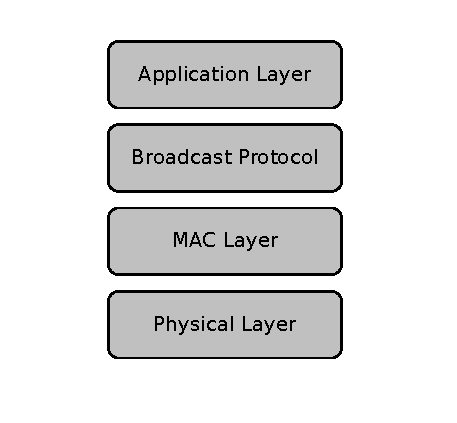
\includegraphics[scale=0.9]{Etat_de_l'art/source/layer.pdf}
\caption{\label{Layer} Les couches dans les réseau de capteur sans fils}
\end{figure}

Pour l'étude et la conception d'algorithmes dans les réseaux de capteurs sans fil (réseau de capteur sans fil), il est indispensable de définir le problème précis, d'établir un cadre rigoureux, formel et sans ambiguïtés.
 Au vue de la figure \ref{Layer}, notre étude se placera dans la couche 'Broadcast Protocols'. Nous ne développerons pas la couche MAC ni la couche application.

Dans le cadre de notre travail d'étude et de recherche, nous utiliserons, sauf mention du contraire, la modélisation de capteurs simplifiée $M_2$ (cf \ref{modelePratique}) avec pour modèle énergétique celui décrit ci dessous.

\subsection{Modèle d'un réseau de capteurs : un graphe}

 \paragraph*{} Un réseau de capteur sans fil peut être représenté par un graphe $G= (V,E,\gamma)$ où :
 \begin{itemize}
 \item $V$ est un ensemble de noeuds (capteurs)
 \item $E \subseteq V \textsuperscript{2}$ est l'ensemble des arêtes représentant les communications possibles entre les capteurs: $(u,v)$ appartient à $E$ signifie que $v$ est à portée de $u$
 \item $\gamma$ est le rayon d'émission maximum
 \end{itemize}
 
 
%%%%%%%%%%%%%%%%%%%%%%%%%%%%%%%%%%  Distance

\begin{mynot}
Soit $ n=|V| $ la taille du réseau de capteur sans fil. Notons que les éléments de E dépendent de la position des capteurs ainsi que de leur portée. Tout les capteurs ont la même portée maximale notée $\gamma$. 
Soit $ij$ l'arête allant de $i$ à $j$. 
Soit $d(u,v)$ la \textit{distance euclidienne} dans $\mathbb{R} \textsuperscript{2}$ entre $u$ et $v$
\end{mynot}
Nous avons:
$$E = \{ (u,v) \in V ^{2} \mid d(u,v) \leq \gamma \}$$

\begin{mydef}
Soit $d_G(u,v)$ la \textit{distance unitaire} entre $ u $ et $ v $ : $d_G(u,v)$ est la taille du plus court un chemin $c(u,v)$ en terme du nombre d'aretes parcourues. 
\end{mydef}


%%%%%%%%%%%%%%%%%%%%%%%%%%%%%%%%%%   Graphe unité&Disque
\begin{mydef}
 Soit $G= (V,E,\gamma)$ le \textit{graphe Unité} du réseau de capteur sans fil et $\gamma$ son rayon de communication (cf fig.\ref{Unit} (a)).
\end{mydef}
\begin{mydef}
Nous définissons le \textit{graphe Disque} comme $G= (V,D,\gamma)$ où $D=\{ Cercle(u,\gamma), u\in V\}$ (cf fig.\ref{Unit} (b)).
\end{mydef}


\begin{figure}[tb]
    \centering
    \begin{tabular}{cccc}
      
      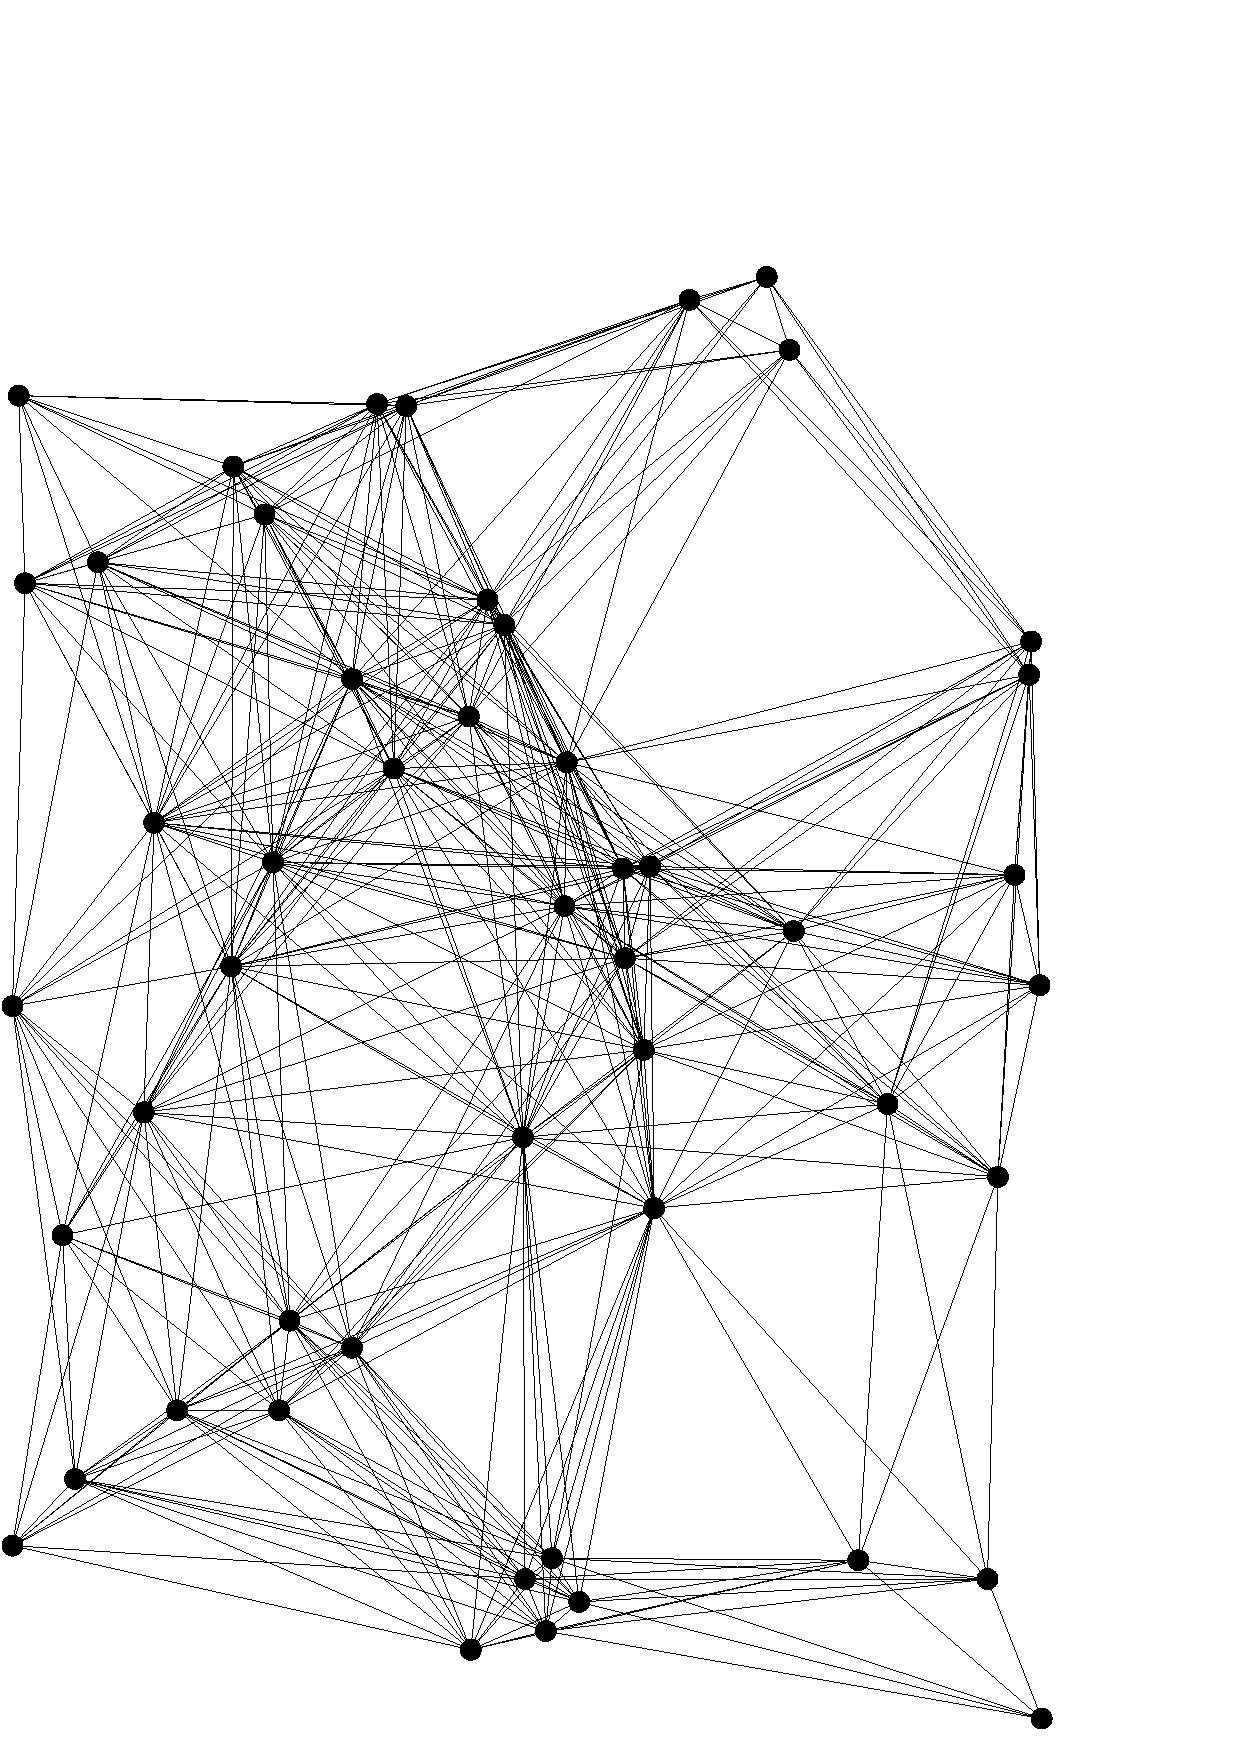
\includegraphics[angle=90, scale= 0.5,width=.5\linewidth]{Etat_de_l'art/source/GrapheUnit.pdf} &
      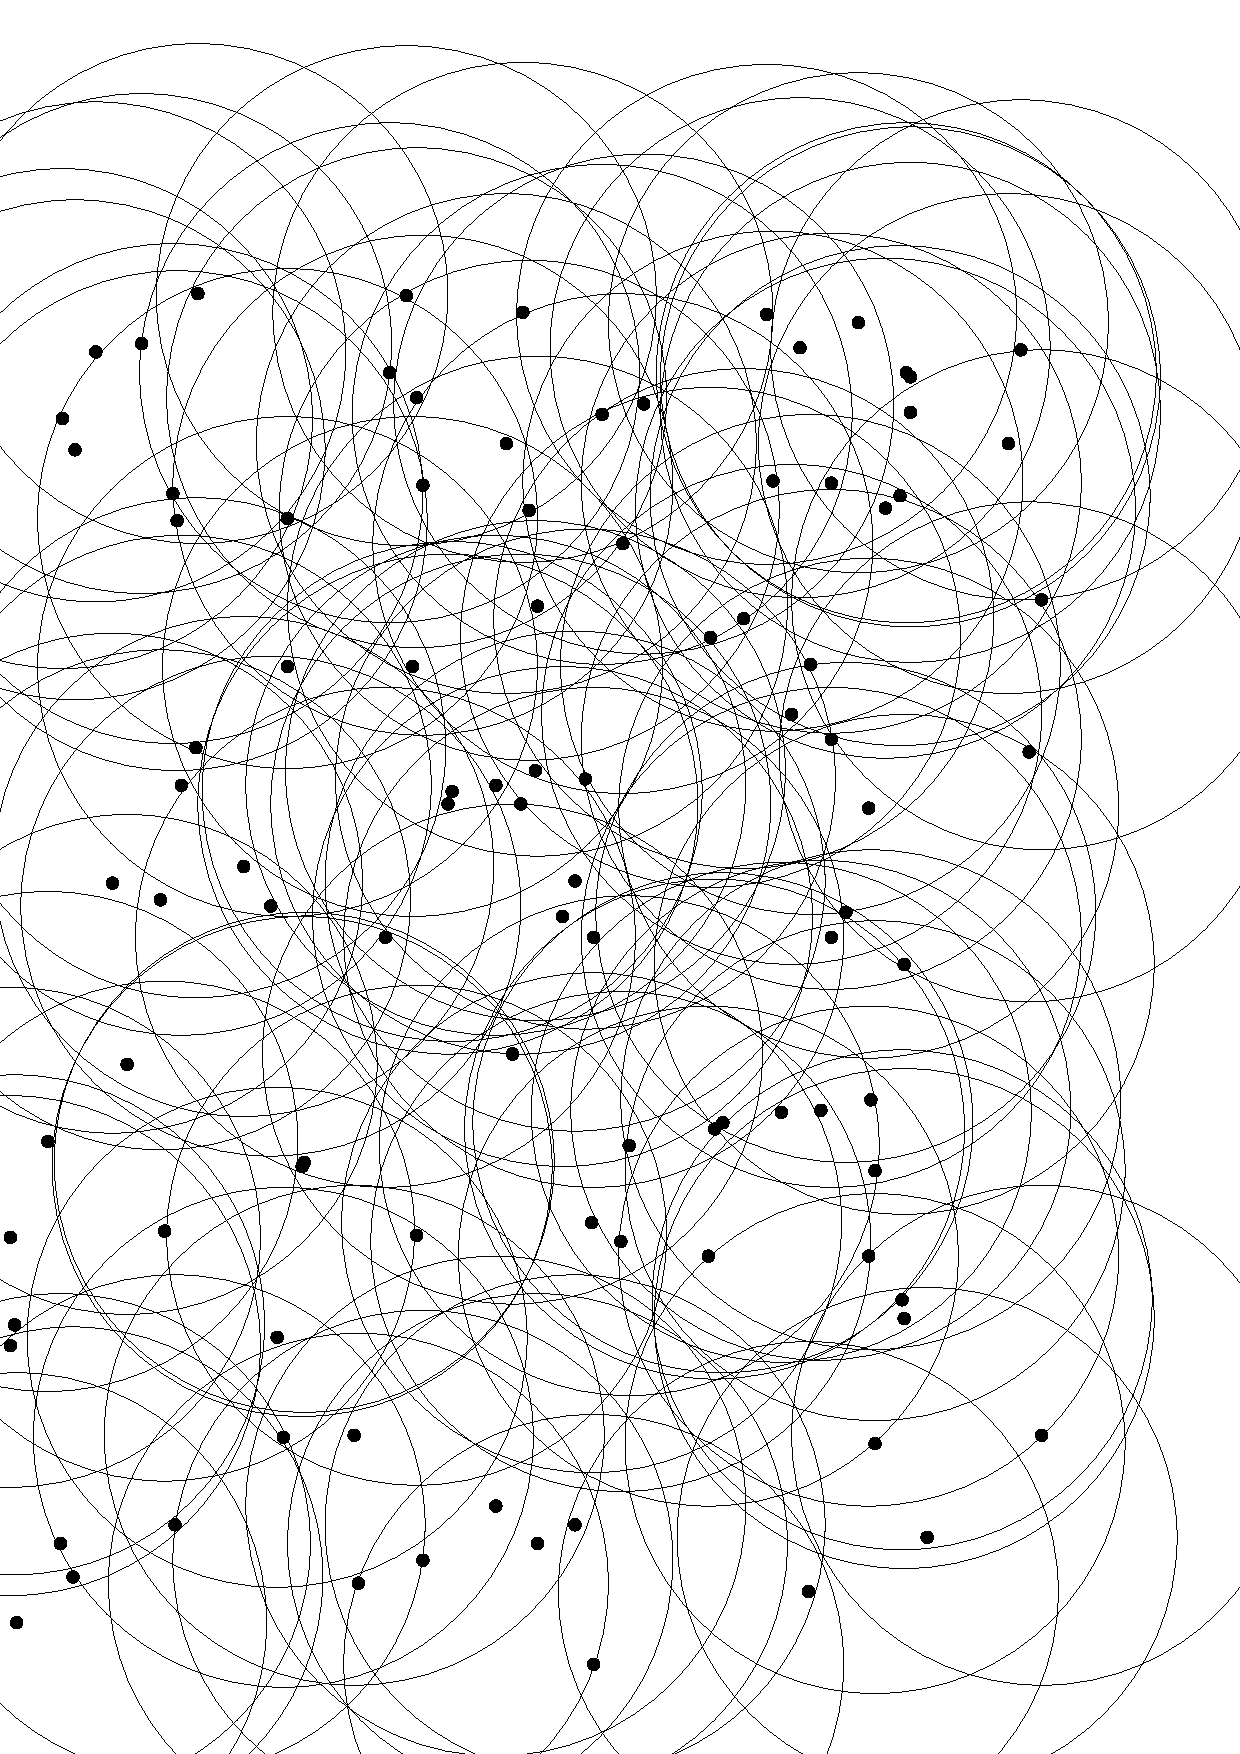
\includegraphics[angle=90, scale= 0.5,width=.5\linewidth]{Etat_de_l'art/source/GrapheUnitDisk.pdf} 
   \\
      (a) & (b) \\
    \end{tabular}
    \caption{Graphe Unité(a) et Graphe Disque(b) \label{Unit}}
\end{figure}

%%%%%%%%%%%%%%%%%%%%%%%%%%%%%%%%%%   Voisinage
\begin{mydef}
Soit $N_1(u)$ le 1-voisinage de $u$ : $N_1(u) = \{ v \in V  \mid (u,v) \in E \}$.
\end{mydef}
\begin{mydef}
Soit $N_1(u)$ le 2-voisinage de $u$ : $N_2(u) = \{ v \in V \mid  \exists w \in V :\{(u,w);(w,v)\} \in E ^2\}$.
\end{mydef}
\begin{mydef}
Soit $N_1(u)$ le $k$-voisinage de $u$, $k \in \mathbb{N} : N_k(u) = \{ v \in V  \mid d_G(u,v)=k \}$.
\end{mydef}
\begin{myvoc}
Nous parlerons de 1- 2- et k-voisins de $i$ pour désigner des noeuds appartenant respectivement
 à $N_1(i), N_2(i),N_k(i)$. 
\end{myvoc}
\begin{mydef}
Le voisinage de  $A \subseteq V$ est l'ensemble $N(A) = \{ v \in V\textbackslash  A \mid \forall u\in A,(u,v) \in E \}$ .
\end{mydef}
\begin{mydef}
Le degré de $ u $ est le nombre  $N(u)=|N_1(u)|$.
\end{mydef}

%%%%%%%%%%%%%%%%%%%%%%%%%%%%%%%%%%   Diametre
\begin{mydef}
Le diametre de $G$ est  $diametre_G= \max\limits_{i,j\in \textlbrackdbl 1,n \textrbrackdbl,i<j} (d_G(i,j))$.
\end{mydef}
 

%%%%%%%%%%%%%%%%%%%%%%%%%%%%%%%%%  Densité, distance moyenne
\begin{mydef}
 Le degré de $G$ est la moyenne des degrés de chaque sommet : $$N_G=\sum_{i=1}^n{\frac1n N(i)}$$.
\end{mydef}
\begin{mydef}
 La densité de $G$ est le nombre $D_G=N_G/diametre_G$.
\end{mydef}
\begin{mydef}
 La distance unitaire de $G$ est la moyenne des distances entre toutes paires de sommets:$$d_G=\sum_{i,j\in \textlbrackdbl 1,n \textrbrackdbl,i<j}{\frac1n d_G(i,j)}$$
\end{mydef}
\begin{mydef}
 La distance euclidienne de $G$ est la moyenne des distances euclidienne entre toutes paires de sommets:$$d(G)=\sum_{i,j\in \textlbrackdbl 1,n \textrbrackdbl,i<j}{\frac1n d(i,j)}$$
\end{mydef}

%%%%%%%%%%%%%%%%%%%%%%%%%%%%%%ù RNG& MST
\begin{mynot}
Nous notons $MST(G)$ un des arbres couvrants de poids minimum de G.
\end{mynot}
\begin{mydef}
Soit $RNG(G)$(pour Relative Neighborhood Graph) le graphe de voisinage .
 $RNG(G)=(V,E_{rng})$ avec $$E_{rng}=\{ (u,v)\in E \mid \nexists w\in N_1(u)\cap N_1(v): d(u,w)<d(u,v) \wedge d(v,w)<d(u,v)  \}$$
Le graphe de voisinage est noté $RNG(G)$ (pour Relative Neighborhood Graph).
\end{mydef}
\begin{myrmq}
 De façon intuitive, pour construire le graphe RNG, pour chaque noeud $u,(u,v)$ est ajouté à $E_{rng}$ si $u$ n'a pas de voisin $w$ plus proche de $v$.
 \end{myrmq}
\begin{myprop}
Nous avons la propriété suivante: $$  MST\subseteq RNG(G)\ \subseteq G$$
\end{myprop}

\begin{figure}[tb]
    \centering
    \begin{tabular}{cccc}
      
      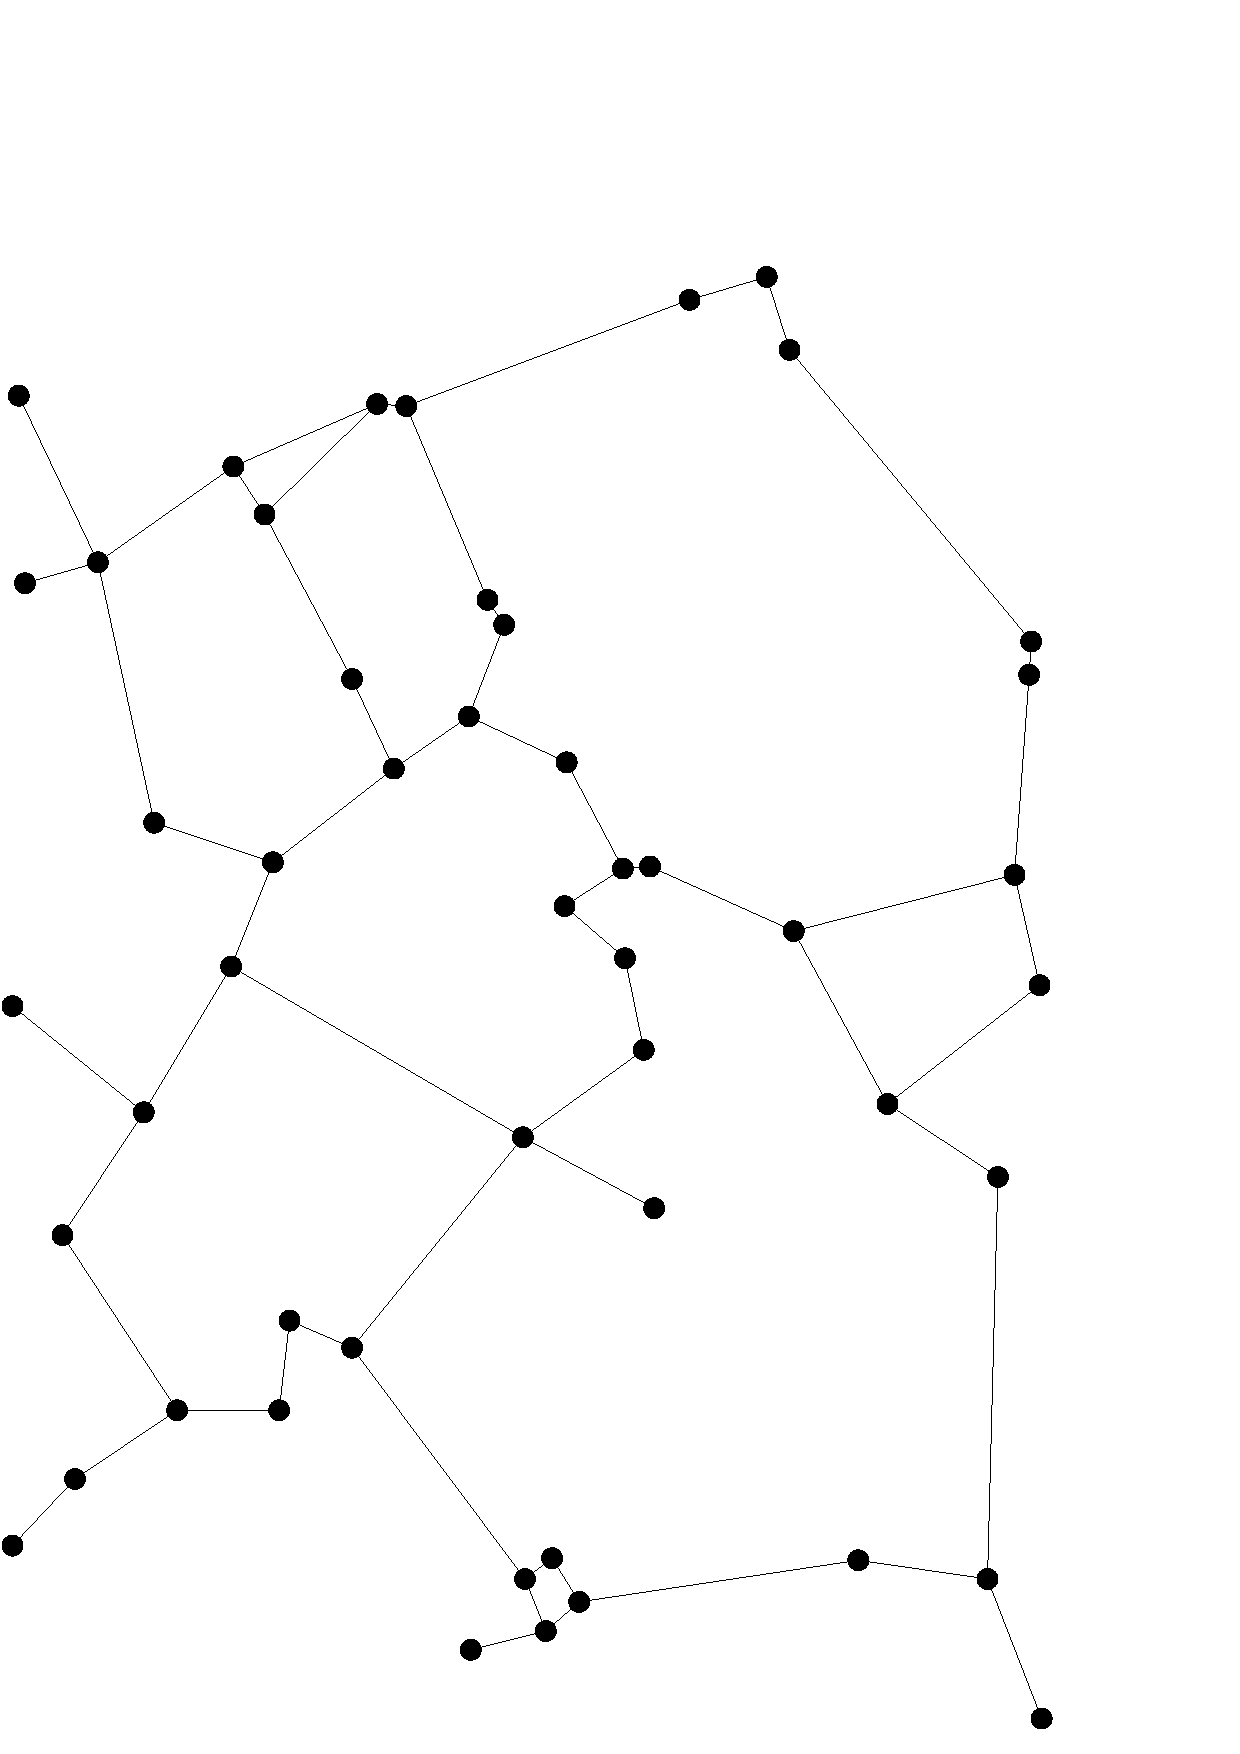
\includegraphics[angle=90, scale= 0.5,width=.5\linewidth]{Etat_de_l'art/source/GrapheRNG.pdf} &
      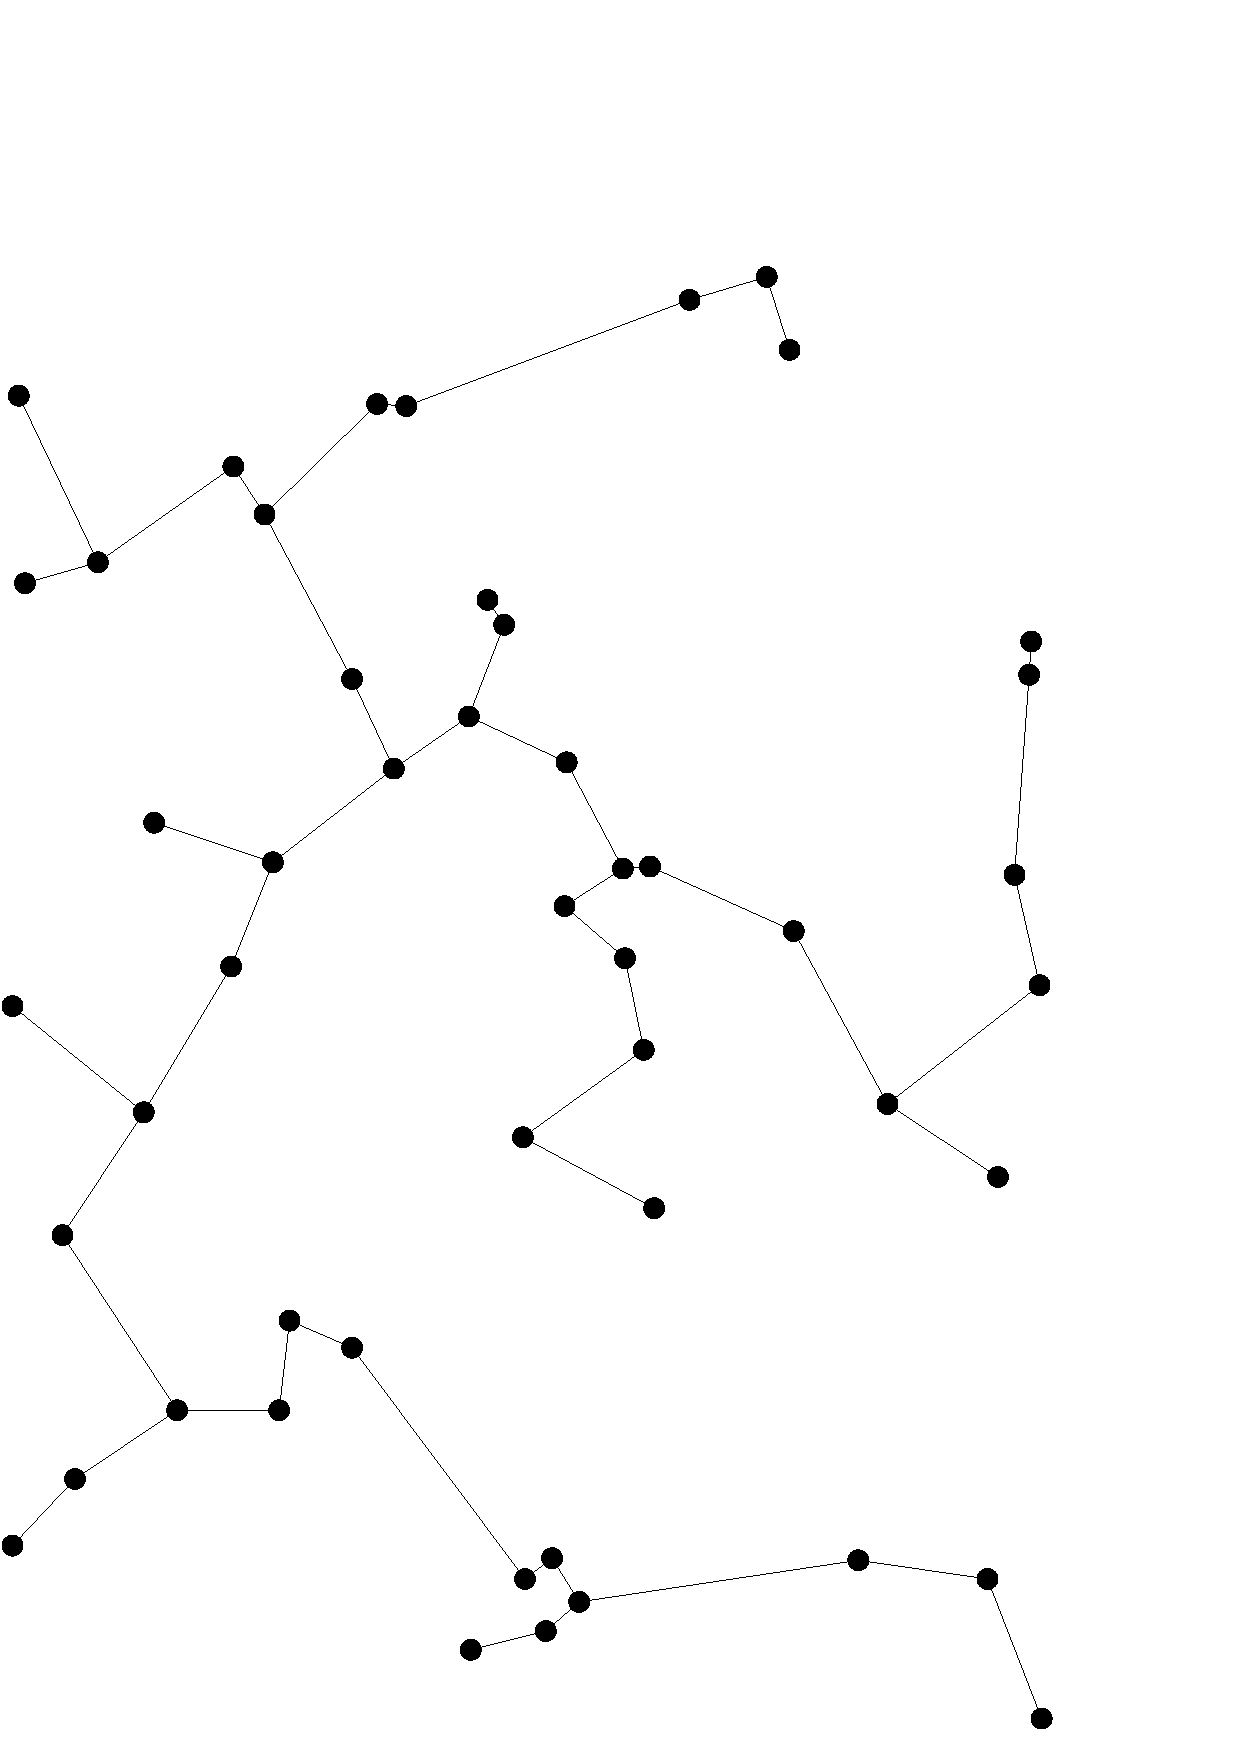
\includegraphics[angle=90, scale= 0.5,width=.5\linewidth]{Etat_de_l'art/source/GrapheMST.pdf} 
   \\
      (a) & (b) \\
    \end{tabular}
    \caption{Graphe RNG(a) et Graphe MST(b) \label{fig:ex}}
\end{figure}


\subsection{Modèle énergétique}
\subsubsection{Energie d'un capteur}
Dans \cite{Dong2005}, Dong présente les deux modèles de consommation énergétique communément utilisés.
\paragraph{The Packet based model.\label{packet_based_model}}
Nous utiliserons pour notre analyse le modèle de consommation d'énergie idéal suivant:
nous considèrerons que chaque capteur $i$ a une énergie initiale $E_{init}=\beta$.
L'envoi de message est le seul facteur de perte d'énergie. L'énergie consommée lors de la réception de message, l'acquisition et traitement des informations sera considérée comme négligeable.
Tous les capteurs $i$ offrant les mêmes caractéristiques, ils peuvent modifier leur rayon d'émission $r_i$ en respectant l'inégalité suivante : $0 \leq r_i \leq \gamma$.
Nous noterons $E_i$ l'énergie restante de $i$.
L'envoi d'un message de $i$ avec un rayon $r$ coûte $$ E(r)= \begin{cases} r^\alpha + c & \text{si }i\neq j \\ 0 & \text{sinon}  \end{cases}$$
L'envoi d'un message de $i$ à $j$ ($d(i,j)\leq \gamma$) coûte  $ E_{ij}=E(d(i,j))$.

\paragraph{The Time based model.}
Ce modèle plus réaliste prend en compte l'énergie de réception des messages, de traitement ainsi que d'écoute inactive du réseau (mode veille).
En effet, dans \cite{Kasten2001}, Kasten souligne le fait que souvent, la réception, l'écoute et le traitement consomment en moyenne autant d'énergie que la transmission de message.
Dans de nombreuses topologies, si la fréquence des transmissions est faible, beaucoup de capteurs vont être à court d'énergie avant même d'avoir pu transmettre des messages.
Dans beaucoup d'applications, la densité du réseau étant élevée, le coût propre aux transmissions de message est relativement faible tandis que le coût de réception des messages est élevé puisque chaque capteur traite les messages de son voisinage (qui en l'occurence est grand).



\paragraph{Energie du réseau.}
\begin{mydef}
 L'énergie potentielle de G est la somme des énergies des capteurs :$$E_G=\sum_{i=1}^n{E_i}$$
\end{mydef}
\begin{mydef}
 La consommation de  G est :$$C_G=n\beta - E_G$$
\end{mydef}
\begin{mydef}
 Le coût moyen de transmission de  G est :$$c_G=E(d(G))$$
\end{mydef}
\begin{mydef}
 Le cout moyen d'une transmission est $C(1)$.\\
 Le cout moyen de $k$ transmissions est $C(k)$.
\end{mydef}


\subsection{Durée de vie du réseau}
\subsubsection{Problématique}


Dans un réseau de capteurs sans fil, la contrainte majeure est l'efficacité de l'algorithme utilisé en matière de consommation énergétique. En effet, la principale caractéristique des capteurs
est leur petite taille et leur micro-batterie. Dans la majeure partie des cas, remplacer les batteries est impossible. Cependant la durée de vie d'un réseau de capteur sans fil est difficile à définir et à mesurer.
Il n'y a pas de définition absolue. Elle indique combien de temps le réseau sera 'efficace' par rapport à l'application donnée (nombre de transmissions effectuées, connexité du réseau, pourcentage de noeuds vivants...).

Dans la littérature, deux approches apparaissent clairement en matière de maximisation de la durée de vie des réseau de capteur sans fils. Une approche indirecte consiste à minimiser la consommation d'énergie de façon locale tandis que l'autre a pour but 
de maximiser la directement la durée de vie du réseau de façon plus globale. Bien que l'approche indirecte puisse améliorer la durée de vie du réseau, elle ne suffit pas à elle seule à appréhender le problème de la durée de vie.
Parmi ces approches figurent  par exemple le fait de maximiser le nombre de transmissions effectuées avant qu'un capteur ne meurt.

Dans \cite{Liang2002}, Liang prouve que le  problème 'THE MINIMUM-ENERGY BROADCAST
TREE PROBLEM' est NP-complet par réduction à (3-CNF SAT):
\begin{myth}
Soient un réseau de capteur sans fil $G$ dans lequel chaque noeud a $k$ rayons de transmission possibles, une source $s$ et un entier positif $w$.
Déterminer s'il existe un arbre de broadcast de source $s$ tel que la somme des coûts de transmission aux noeuds relais (qui ne sont pas des feuilles) soit inférieure à $w$ est NP-Complet.
\end{myth}
Ainsi, pour un broadcast donné il n'existe pas d'algorithme centralisé polynomial pour trouver l'arbre de diffusion optimale. Il est évident qu'il n'en existe pas de distribués. 
Dans \cite{Dong2005}, Dong prouve que le  problème BROADCAST LIFETIME est NP-Complet par réduction à (3DM):
\begin{myth}
Soient un réseau de capteur sans fil $G$, une source $s$ et un entier positif $k$.
Déterminer si G a assez d'énergie pour broadcaster $k$ messages a partir de $s$ est NP-Complet.
\end{myth}

De façon formelle, il est donc souvent impossible de calculer le nombre total de broadcasts réussis étant donné un réseau et un protocole (sauf quand le protocole est très simple). Nous analyserons donc \textit{les performances moyennes} des algorithmes quand cela est possible. Sinon, les simulations nous permettront de mesurer les performances en fonction de différentes topologies.

\subsubsection{Définitions}
Les définitions et critères de durée de vie d'un réseau de capteur sans fil sont tirés des articles \cite{Dietrich2009},\cite{Champ2009lifetime},\cite{Elleithy2011}. 

\begin{mylt}\label{TTFF}
Nombre moyen de transmissions réussies avant qu'un capteur n'ai plus de batterie (TTFF).
\end{mylt}
\begin{mylt}\label{LC}
Nombre moyen de transmissions réussies avant que le réseau ne perde sa connectivité (LC).
\end{mylt}
\begin{mylt}\label{PCN}
Nombre moyen de transmissions réussies jusqu'à ce qu'il ne reste que $X\%$ de noeuds vivants (PCN).
\end{mylt}


%TODO Reduire taille tableau
\begin{table}[H]
{%
\newcommand{\mc}[3]{\multicolumn{#1}{#2}{#3}}
\begin{center}
\begin{tabular}{|c|l}
\hline
$G(V,E,\gamma)$ & \mc{1}{c|}{Graphe unité}\\\hline
$n$ & \mc{1}{c|}{Nombre de capteurs}\\\hline
$\gamma$ & \mc{1}{c|}{Rayon d'émission maximum}\\\hline
$\alpha$ & \mc{1}{c|}{Constante de consommation énergetique}\\\hline
$c$ & \mc{1}{c|}{Constante de consommation énergetique}\\\hline
$\beta$ & \mc{1}{c|}{Energie initiale des capteurs}\\\hline
$E_i$ & \mc{1}{c|}{Energie restante de $i$}\\\hline
$E_{ij}$ & \mc{1}{c|}{Coût d'envoi d'un message de $i$ à $j$}\\\hline
$N(u) $& \mc{1}{c|}{Degré de u}\\\hline
$d_G(i,j)$ & \mc{1}{c|}{Distance dans G entre $i$ et $j$}\\\hline
$d(i,j)$ & \mc{1}{c|}{Distance euclidienne entre $i$ et $j$}\\\hline
$N_k(u)$ & \mc{1}{c|}{Nombre de k-voisins de u }\\\hline
$N_G$ & \mc{1}{c|}{Degré de G}\\\hline
$d_G$ & \mc{1}{c|}{Distance de G}\\\hline
$d(G)$ & \mc{1}{c|}{Distance euclidienne de G}\\\hline
$diametre_G$ & \mc{1}{c|}{Diametre de G}\\\hline
$D_G$ & \mc{1}{c|}{Densité de G}\\\hline
$C(k)$ & \mc{1}{c|}{Coût de $k$ broadcasts}\\\hline

\end{tabular}
\end{center}
}%
\caption{Notations}
\end{table}



\section{Eléments de classification des algorithmes existants}\label{class}

Les éléments de classification cités ci-dessous sont inspirés des articles \cite{stojmenovic2004}, \cite{ingelrest2005}, \cite{wu2003}.



\subsection{Transmissions en broadcast vs transmissions en single-cast}
Dans un réseau $G(V,E,\gamma)$, deux capteurs peuvent communiquer directement uniquement s'ils sont 1-voisins dans G. A cause l'atténuation du signal wifi, le rayon de transmission est relativement limité, c'est pourquoi les communications doivent se faire par multi-sauts. Tout ceci est géré par un algorithme de routage. Les algorithmes de routage peuvent gérer le broadcast (un nœud vers tous les autres) et/ou le single-cast (un nœud vers un autre). Chacune des approches a des avantages dans un contexte précis.

\subsubsection{Broadcast}
La procédure de broadcast consiste à transmettre une information à tous les autres nœuds du graphe. C'est un mécanisme fondamental pour la propagation des données ainsi que pour la découverte de routes. En effet le broadcast est utilisé pour acquérir une connaissance du voisinage des capteurs. Ce mode de communication est naturel pour des périphériques en wifi avec antenne omnidirectionnelle car les ondes sont réparties uniformément dans un cercle de rayon donné. Tout le voisinage est donc touché et le coût en énergie est celui d'une seule transmission.

Le routage des broadcasts nécessite de s'assurer que le message ne soit pas indéfiniment retransmis mais que tous les nœuds du graphe soient touchés. Parfois même si le destinataire est à distance 1 dans le graphe unité, il est nécessaire que le message soit relayé par un nœud tiers pour des raisons énergétiques.

\subsubsection{Single-cast}
La transmission par single-cast est le moyen classique de transmettre les messages : un expéditeur fait parvenir un message à un destinataire. Ce moyen de communication est valable lorsqu'on ne cherche qu'à atteindre un seul nœud. En effet, le routage d'un single-cast coûte moins cher que le broadcast (en moyenne, moins de transmissions sont nécessaires).


\subsection{Algorithme à rayon d'émission fixe vs variable}
Dans les réseaux de capteurs, les transmissions s'effectuent sans fils. Un bon moyen de réduire la quantité d'énergie utilisée est donc de réduire la portée d'une transmission. L'idée des algorithmes de broadcast est de choisir les noeuds relais de façon à ce que leur ensemble se rapproche au maximum d'un maillage optimal. Certains algorithmes choisissent de fixer un rayon égal pour tous les nœuds ; d'autres utilisent un rayon variable pour chaque nœud. 

Notons que les algorithmes qui émettent en single-cast ont, par définition, un rayon d'émission variable.

\subsubsection{Déterminer le rayon optimal d'émission pour un broadcast}
\begin{myth}
Sans chevauchement et sans vide, un plan ne peut être découpé de façon uniforme que par des polygones réguliers de type triangle, carrés ou hexagones.
\end{myth}
\begin{proof}
Soit $m$ le nombre de sommets d'un $m$-polygone et $n$ le nombre de $m$-polygones nécessaires pour couvrir $2\pi$ degrés. La somme des angles internes étant égale au produit d'un 
angle interne par le nombre de côtés $m$, elle sera égale à $\pi m-2 \pi$  radian. Un angle interne vaut donc $\frac{(m-2)\pi }{m}$ . Nous avons: 
$$\frac{(m-2)n\pi}{m}=2\pi \Leftrightarrow (m-2)(n-2)=4$$
Comme $n$ et $m$ sont des entiers, les seules solutions sont : 
$$(m-2;n-2)\in\{(1,4),(2,2),(4,1) \} \Leftrightarrow m \in \{ 3,4,6 \}$$
\end{proof}

\begin{myth}
Le quadrillage en hexagone est celui offrant le moins de chevauchements du point de vue réseau de capteur sans fil. 
\end{myth}
\begin{proof}
 %TODO
\end{proof}



Soit $P$ un plan sur lequel $n$ capteurs sont placés. Chaque capteur peut émettre des messages avec un rayon compris entre 0 et $\gamma$. Nous allons déterminer pour tous les nœuds un même rayon d'émission fixe $R$.
Etant donnée une source $s$ et un message $M$ à broadcaster, nous devons placer les noeuds relais de façon à minimiser leur nombre $m$. Bien sûr, leur nombre dépend directement du rayon $R$.
 

Dans un réseau hexagonal, nous avons les résultats suivants :
Soit $S$ l'aire du plan rectangulaire $P$. Connaissant $R$, nous pouvons calculer facilement le nombre de sommets nécessaires pour couvrir le plan.
Soit $h$ le nombre d'hexagones couvrant $P$, on a : 
$$h \simeq \frac{Surface ( P)}{Surface(hexagone)}=\frac{2S}{3R^2 \sqrt{3}}$$

Comme il faut deux nœuds par hexagone,
\begin{eqnarray*}
n & = & 2h \label{eq:3}\\
 & = & \frac{4S}{3R^2 \sqrt{3}}\\
 & = & \frac{k}{R^2}\label{eq:4}
\end{eqnarray*}

Ainsi, le coût d'un broadcast vaut:
\begin{eqnarray*}
C(1)(R) & = & 2h \label{eq:3}\\
 & = & n\cdot E(R)\\
 & = & \frac{k}{R^2}\cdot E(R)\\
 & = &  \frac{k}{R^2}\cdot (R^\alpha+c) \label{eq:4}
\end{eqnarray*}
 
Nous cherchons le rayon optimal minimisant $C(1)(R)$. Comme $\alpha\geq 2$, $c\geq 0$ et $R>0$, nous avons 4 cas possibles:
\begin{itemize}
 \item $\alpha=2$, $c=0$:  $C(1)(R)=k$. $R_{opt}$ ne dépend pas de $r$.
 \item $\alpha=2$, $c\neq0$: $C(1)(R)=k(1+cR^{-2})$. Le rayon doit être le plus grand possible donc : $R_{opt}=\gamma$.
 \item $\alpha>2$, $c=0$: $C(1)(R)=kR^{\alpha-2}$. $R_{opt}=0$
 \item $\alpha>2$, $c\neq 0$: $C(1)(R)=k(R^{\alpha-2} + c R^{-2} ) $.\\
 En dérivant, nous obtenons: $C'(1)(R)= k( (\alpha-2) R^{\alpha-3}- 2cR^{-3} ) $.\\
Cette fonction admet un minimum en $$R_{opt}=\sqrt[\alpha]{\frac{2c}{\alpha-2}}$$
\end{itemize}

Bien sûr, en pratique il est impossible, sur une topologie quelconque, d'extraire un tel maillage hexagonal de rayon $R_{opt}$. Cepandant il est possible de s'en approcher le plus possible.


\subsubsection{Rayon d'émission fixe pour tous les nœuds}
Certains algorithmes de broadcast les plus primitifs ($cf$ \ref{blind_flooding}, \ref{proba_flooding}) utilisent un rayon d'émission fixe. Les performances énergétiques associées ne sont pas très bonnes car réduire le rayon d'émission et réduire le nombre de transmissions sont les deux seuls moyens d'économiser de l'énergie lors du routage d'un broadcast.


\subsubsection{Rayon d'émission variable}
La plupart des algorithmes  de broadcast utilisent un rayon d'émission variable pour les raisons citées ci-dessus. Tous les algorithmes de routage de single-cast utilisent un rayon d'émission variable car ils ajustent leur transmission pour toucher uniquement le nœud destinataire.



\subsection{Algorithme global vs local}
Le fait qu'un algorithme soit global ou local dépend du type d'informations qu'il utilise. Si un capteur connait dès son arrivée des informations sur ses voisins, l'algorithme est global. À l'inverse, un algorithme distribué fournit aux capteurs uniquement les informations que leurs perceptions peuvent leur procurer.

Cependant, la distinction entre global et local n'est pas toujours évidente. Des algorithmes centralisés peuvent être implémentés d'une manière distribuée en décidant par exemple d'un noeud possédant la connaissance globale du réseau. À l'inverse, un algorithme distribué peut simuler une connaissance globale : au travers d'un échange séquentiel et très localisé d'informations  (1 ou 2-voisinage par exemple), chaque noeud peut combiner sa connaissance avec celle de ses voisins et ainsi obtenir une vision globale du réseau. Cependant, une telle phase de propagation coûte très cher en terme de nombre de messages échangés et de temps.

Si le réseau est dynamique (mobilité des capteurs), maintenir une connaissance locale du réseau devient plus complexe tandis que tenir à jour la topologie globale de celui-ci devient impossible par le moyen cité précédemment. Ainsi, la quantité et la nature des informations nécessaires au déroulement de l'algorithme sont une bonne mesure de la capacité d'adaptation du protocole à un environnement dynamique.   

\subsubsection{Catégories}
\begin{description}
 \item[Global :]protocole de routage, centralisé ou distribué nécessitant une connaissance globale du réseau.
 \item[Quasi-global :]protocole distribué de broadcast nécessitant une connaissance quasi-globale du réseau.
 \item[Quasi-local :]protocole distribué nécessitant une connaissance du réseau principalement locale et occasionnellement globale (ex: Cluster networks: tandis que les groupes peuvent être construits de manière locale, des réactions en chaines peuvent arriver).
 \item[Local :]protocole distribué nécessitant une connaissance très locale du réseau. Tous les algorithmes de 1 ou 2-voisinage appartiennent à cette catégorie.
\end{description}

Remarquons que pour qu'un protocole soit extensible, il doit être avant tout distribué et local :  le comportement de chaque noeud, bien qu'il nécessite qu'une connaissance locale du réseau, permet d'atteindre l'objectif global. Il est facile d'admettre que l'extensibilité d'un réseau de capteur sans fil est inversement proportionnelle à la localité du protocole.



\subsection{Algorithme à balisage vs algorithme sans balisage (beaconless)}
Les algorithmes ``beaconless'' ne nécessitent pas de phase d'initialisation ni de mise à jour. Les nouveaux capteurs sont immédiatement opérationnels mais n'ont aucune connaissance de leur environnement et notamment de leur voisinage dans G. 

Dans les algorithmes avec balisage, tout capteur, lorsqu'il est connecté au réseau, commence par une procédure d'initialisation et stocke en mémoire un certain nombre d'informations (voisins, groupe, topologie locale...). Au cœur de l'algorithme, chaque noeud met périodiquement à jour ces informations. Il est possible, par exemple, que chaque site envoie régulièrement à ses voisins un message de type
'Hello' contenant par exemple son Id, sa position, sa dominante connexe, son degré, ses voisins, etc.



\subsection{Algorithme déterministe vs probabiliste}
Un algorithme déterministe est un algorithme qui, confronté à un choix, prendra toujours la même décision : celle prévue par le concepteur. Chaque nœud prendra donc, dans des conditions similaires, la même décision.

À l'inverse, un protocole de routage peut utiliser des fonctions probabilistes pour prendre certaines décisions de manière aléatoire. Il en existe deux types : l'un qui prend toujours la décision optimale mais au bout d'un temps qui peut être long ; l'autre qui décide rapidement mais dont la décision peut être mauvaise.



\section{Quelques algorithmes de routage}
Tous les algorithmes présentés ci-dessous utilisent la modélisation $M2$ (\ref{modelePratique}) des réseaux avec pour modèle énergétique le 'Packet based model' (\ref{packet_based_model}).


\subsubsection{Flow augmentation \cite{Chang2000}}

\emph{Description :}
L'algorithme $FA(x_1, x_2, x_3)$ est un algorithme d'augmentation de flot. L'idée consiste à utiliser un algorithme de plus court chemin existant (comme l'algorithme distribué de Bellman-Ford) et de lui passer trois paramètres ($x_1$, $x_2$ et $x_3$) qui détermineront sa fonction de poids sur les arcs. Ces paramètres coefficienteront les trois facteurs suivants : le coût de transmission du nœud $i$ au nœud $j$ ($e_{ij}$) ; l'énergie résiduelle du nœud $i$ ($\underline{E}_i$), et l'énergie initiale du nœud $i$ ($E_i$). Voici la formule qui donne le poids de l'arc $(i,j)$ en fonction des paramètres :
\begin{displaymath}
c_{ij} = e_{ij}^{x_1} \underline{E}_i^{-x_2} E_i^{x_3}
\end{displaymath}

\begin{algorithm}[H]
\caption{$FA(x_1,x_2,x_3)$}
\label{algo_FA}
\begin{algorithmic}
\REQUIRE a network $ G(N,A) $

\WHILE {each node $i$ has some energy}
	\FOR {each commodity $c \in C$}
		\FOR{each origin node $o \in O^{(c)}$}
			\STATE compute the shortest cost path from $o$ to $D^{(c)}$
			\STATE augment the flow on this path by an amount of $\lambda Q_i^{(c)}$
		\ENDFOR
	\ENDFOR
\ENDWHILE

\RETURN the total flow q in the network
\end{algorithmic}
\end{algorithm}


\emph{Durée de vie} :  $$TTFF(q) = \min\limits_{i \in N}\frac{E_i}{\sum \limits_{j \in S_i} {e_{ij}} \sum \limits_{c \in C} {q_{ij}^{(c)}}}$$
avec :
\begin{itemize}
\item $q$ le flot
\item $N$ l'ensemble des nœuds du graphe (les capteurs)
\item $E_i$ la quantité d'énergie initiale du nœud $i$
\item $S_i$ l'ensemble des voisins du nœud $i$
\item $e_{ij}$ l'énergie requise pour transmettre une unité d'information du nœud i au nœud j
\item $C$ l'ensemble des composantes du réseau
\item $q_{ij}^{(c)}$ le taux d'information de la composante c transmise du nœud $i$ au nœud $j$
\end{itemize}



\subsubsection{Flow redirection \cite{Chang2000}}


\emph{Description :}
Cet algorithme est basé sur le fait que le flot trouvé est optimal ssi pour tous les chemins de l'origine à la destination portants un flot positif, la durée de vie minimum est la même. Le principe consiste donc à rediriger une partie du flot de chaque nœud à travers un autre chemin vers la destination tel que la durée de vie de chaque chemin portant du flot augmente (ou au moins reste stable). Le flot initial a pour valeur la quantité totale d'informations générées par le réseau.

Pour chaque nœud dans le réseau, on compare les chemins sortants de ce nœud vers la destination. On construit un ordre total sur ces chemins en les classant en fonction de leur nœud qui possède la plus courte durée de vie (puis par nombre de nœuds).

Si le nœud dont la durée de vie est la plus courte sur le chemin est le nœud source ($i$), alors on a deux choix. On regarde les voisins sortants de ($i$). Soit on redirige un des flots qui passe par le voisin ($j$) dont le coût de transmission $e_{ij}$ est le plus grand vers un des chemins qui passe par le voisin ($j$) dont le coût de transmission $e_{ij}$ est le moindre. Soit on redirige un flot quelconque vers le chemin le plus petit dans l'ordre total parmi ceux qui passe par le voisin ($j$) dont le coût de transmission $e_{ij}$ est le moindre.

Si, en revanche, le nœud dont la durée de vie est la plus courte sur le chemin n'est pas le nœud source, on a également deux possibilités. Dans les deux cas on redirige le flot le plus petit dans l'ordre total. Soit on redirige vers le chemin le plus grand dans l'ordre total. Soit on redirige vers le chemin qui passe par le voisin ($j$) dont le coût de transmission $e_{ij}$ est le moindre parmi les chemins supérieurs dans l'ordre total au chemin redirigé.

Une fois que l'algorithme a défini pour un nœud donné les deux chemins, il détermine la quantité de flot à rediriger.

\begin{algorithm}[H]
\caption{$FR()$}
\label{algo_FR}
\begin{algorithmic}
\REQUIRE a network G(N, A)

add to $G$ an imaginary super destination node $\tilde{d}^{(c)}$
\FOR{all $d \in D^{(c)}$}
	\STATE $\tilde{d}^{(c)} \in S_d$
	\STATE $e_{d \tilde{d}^{(c)}} = 0$
\ENDFOR

let $q$ be the initial flow
\FOR{all $o \in O^{(c)}$}
	\STATE $q_{o \tilde{d}^{(c)}} = Q_o^{(c)}$
\ENDFOR

\FOR{each $c \in C$}
	\FOR{each $i \in N - D^{(c)}$}
		\STATE (Determine the Two Paths)
		\STATE (Calculate $\epsilon_i^{(c)}$)
		\STATE (Redirect the flow)
	\ENDFOR
\ENDFOR

\RETURN 
\end{algorithmic}
\end{algorithm}



\emph{Durée de vie} :  $$TTFF(q) = \min\limits_{i \in N}\frac{E_i}{\sum \limits_{j \in S_i} {e_{ij}} \sum \limits_{c \in C} {q_{ij}^{(c)}}}$$



\subsubsection{Energy Aware Routing \cite{Shah2002}}

\emph{Description :}
Ce protocole est réactif (càd qu'il ne découvre un chemin entre deux nœuds qu’en cas de besoin) et les requêtes sont initiées depuis la destination. Il se décline en trois phases : la phase d'initialisation qui permet de trouver tous les chemins de la source à la destination ; la phase de communication de données ; et la maintenance des routes. Les deux premières phases sont détaillées dans les algorithmes ci-dessous.

\begin{algorithm}[H]
\caption{Setup phase of EAR}
\label{algo_EAR_sp}
\begin{algorithmic}

\STATE $Cost(N_D) = 0$

\COMMENT{Flood the network from $N_D$ to $N_S$ :}
\FOR{each intermediate node $N_i$}
	\FOR{each neighbor $N_j$ of $N_i$}
		\IF{$d(N_i,N_S) \geq d(N_j, N_S)$ and $d(N_i,N_D) \leq d(N_j, N_D)$}
			\STATE Forward the request from $N_i$ to $N_j$
		\ENDIF
	\ENDFOR
\ENDFOR
\STATE
\FOR{each intermediate node $N_i$}
	\FOR{each neighbor $N_j$ of $N_i$}
		\STATE On receiving a request :
		\STATE $C_{N_j,N_i} = Cost(N_i)+Metric(N_j,N_i)$
		\STATE $FT_j = \{i | C_{N_j,N_i} \leq \alpha (\underset{k}{min}\ C_{N_j,N_k})\}$
		\STATE
		\STATE $P_{N_j,N_i} = \dfrac{\dfrac{1}{C_{N_j,N_i}}}{\sum \limits_{k \in FT_j} \dfrac{1}{C_{N_j,N_k}}}$
		\STATE
		\STATE $Cost(N_j) = \sum \limits_{i \in FT_j} {P_{N_j,N_i} C_{N_j,N_i}}$
	\ENDFOR
\ENDFOR
\end{algorithmic}
\end{algorithm}


\begin{algorithm}[H]
\caption{Data communication phase of EAR}
\label{algo_EAR_dcp}
\begin{algorithmic}

\STATE $N_S$ chooses randomly a number
\STATE This number points a neighbor in the forwarding table $FT_S$ out
\STATE Send the packet from $N_S$ to this neighbor $N_j$
\STATE Do the same thing for all intermediate nodes until the packet reaches the destination

\end{algorithmic}
\end{algorithm}



\section{Quelques algorithmes de broadcast}

\subsubsection{Blind Flooding\label{blind_flooding}}


\emph{Description :} le "blind flooding" ou "broadcast aveugle" est un algorithme glouton de broadcast sans balisage. Lors de la réception d'un message par un noeud, si c'est la première fois qu'il le reçoit, il le broadcast à ses voisins (avec le rayon maximum), sinon il ne fait rien.

\emph{Consommation} :  le coût global d'un broadcast est exactement le coût moyen puisque chaque noeud $i$ envoie un unique message <$M$,$\gamma$> par broadcast.
Le coût global d'un broadcast est $C(1) = n \cdot E( \gamma )= n\cdot \gamma^\alpha +  n\cdot c $.
Le coût global de $k$ broadcasts est $C(k) = k\cdot n \cdot E( \gamma )= k\cdot n \cdot \gamma^\alpha +  k \cdot n\cdot c $.

\emph{Durée de vie} :   $$TTFF(Blind Flooding)=\lfloor \frac{\beta}{n\cdot \gamma^\alpha +  n\cdot c} \rceil$$



\subsubsection{Probabilistic Flooding\label{proba_flooding}}

\emph{Description :} Afin d'éviter le redondance et les collisions, une idée est que chaque noeud retransmette le message suivant une probabilité $P$ lorsqu'il le reçoit pour la première fois. Si $P=1$ cela équivaut au blind flooding.
\emph{Consommation :} Chaque noeud ayant un probabilité $P$ de retransmettre le message <$M$,$\gamma$>, en moyenne $P\cdot n$ nœuds envoient ce message lors d'un broadcast.
Le coût moyen d'un broadcast est $C(1) = P\cdot n \cdot E( \gamma ) $. Le coût global de $k$ broadcasts est $C(k) = P\cdot k\cdot n \cdot E( \gamma ) $ .
\emph{Durée de vie :} $$TTFF(Probabilistic Flooding)=\lfloor \frac{\beta}{P \cdot (n\cdot \gamma^\alpha +  n\cdot c)} \rceil$$


\subsubsection{Area-based Beaconless Broadcasting Algorithms \cite{Ovalle2006}}


\emph{Description :} Nous supposons que les noeuds n'ont aucune connaissance de leur voisinage. Cependant ceux-ci connaissent leur position géographique (GPS par exemple). Chaque capteur a un rayon d'émission fixe $R$ et couvre une zone circulaire.
\begin{figure}[H]
\centering
\includegraphics{Etat_de_l'art/source/abba.png}
\caption{ }
\end{figure} 

L'idée maitresse de ABBA est assez simple. A la première réception d'un message, le nœud initialise un timer. Avant expiration du timer, le noeud peut recevoir d'autres copies du même message. Si un nœud $u$ reçoit le même message de différentes sources et que ces sources couvrent sa zone, cela signifie que chacun de ses voisins potentiels a déjà reçu le message. Alors $u$ ne retransmet pas le message et quand que son timer expire, il ne fait rien. Sinon si le voisinage de $u$ n'est pas couvert alors $u$ retransmet.

Comme chaque couverture est un cercle de rayon $R$, le critère de couverture peut être simplifié : au lieu de s'intéresser au disque entier, un noeud vérifie uniquement si le périmètre $\pi$ de sa zone est couvert par ses voisins lui ayant envoyé le message.


\begin{algorithm}[H]
\caption{ABBA}
\label{ABBA}
\begin{algorithmic}
\REQUIRE:
Un noeud source $s$, un message $M$
\STATE $s$ envoie  <$M$,$s$,$position_s$,$R$> ;
\STATE Réception  par  $u$ de  <$M$,$v$,$position_v$,$R$>
\STATE $z_u\leftarrow ensemble_{vide}$ ;
\STATE Calculer la zone $z$ couverte par $v$ lors de la transmission;
\STATE Déclencher le timer;
\REPEAT
    \STATE Attendre la réception d'un autre copie de $M$ ou que le timer expire;
    \IF {Une copie de $M$ est reçue}
	\STATE Mettre à jour $z_u$;
	\STATE réinitialiser le timer;
    \ENDIF
\UNTIL{timer expire;}
\IF {$\pi \nsubseteq z_u$}
    \STATE Retransmettre;
\ENDIF
     \STATE Ignorer les autres copies de M;

\end{algorithmic}
\end{algorithm}


\subsubsection{Broadcast Incremental-power Protocol \cite{Wieselthier2000}}



\emph{Description :} Rappelons les désavantages des transmissions longue portée: interférences, cout énergétique (le modèle de consommation énergétique des noeuds est non linéaire par rapport au rayon à cause de l'atténuation du signal radio).
C'est pourquoi il est nécessaire de trouver le bon compromis entre le rayon de transmission et le nombre de messages circulant. En effet, un large rayon de transmission coûte cher mais atteint beaucoup de nœuds ; un court rayon coûte très peu cher mais augmente le nombre de messages. 

BIP est glouton et centralisé. Il se base sur l'algorithme de Prim \cite{Prim1957} : un algorithme permettant de construire un arbre couvrant de poids minimum à partir d'un sommet d'un graphe. Le principe de l'algorithme de Prim est de construire l'arbre couvrant minimal arête par arête. Pour ajouter une arête à un arbre partiellement construit, il considère l'ensemble des arêtes dont une extrémité est connectée à l'arbre déjà construit, et l'autre extrémité ne l'est pas. Il choisit dans cet ensemble une arête de poids minimal qu'il ajoute à l'arbre. L'algorithme commence avec un arbre contenant un nœud et pas d'arêtes, et ajoute successivement $n-1$ arêtes.

La formation d'un arbre couvrant de poids minimum dans BIP suit le même principe dans le sens où les arêtes sont une par une ajoutées à l'arbre. En fait, BIP utilise l'algorithme de Prim avec une différence fondamentale : au lieu d'utiliser des coûts fixes $P_{ij}$ sur les arêtes (demeurant inchangés au cours de la procédure), BIP actualise dynamiquement ces couts $P'_{ij}$ à chaque étape ($i.e$ à chaque ajout d'une arête).

Posons $P(i)$ le poids du nœud $i$ qui correspond au coût de broadcast de $i$ dans l'arbre (i.e. : son rayon d'émission actuel). À chaque étape de BIP, les poids des nœuds changent : en effet, à chaque étape on ajoute une arête et on change potentiellement les arêtes déjà choisies. Chaque nœud dans l'arbre de BIP (dont celui nouvellement ajouté) change de poids s'il devient père d'un nouveau nœud qui l'oblige à augmenter son rayon d'émission. On a donc :
$$\begin{cases}
	P(i)=0  & \text{si $i$ est une feuille ou que $i$ n'est pas encore dans l'arbre}\\
	P(i)=\max\limits_{\forall j\in N_1(i)\bigcap BIP}(P_{ij}) & \text{sinon}\\
\end{cases}$$

Le coût d'ajout d'une arête dépend des nœuds déjà dans l'arbre de la façon suivante : 
$$ \forall i \in BIP, \forall j \notin BIP, P'_{ij}=P_{ij}-P(i)$$
où $P_{ij}$ est le coût réel de transmission (poids de l'arête). $P'_{ij}$ représente donc le coût d'ajout de $j$ comme fils du noeud $i$. La paire $\{i,j\}$ minimisant $P'_{ij}$ avec $i \in BIP$ et $j \not\in BIP$ est sélectionnée et $i$ ajuste son rayon pour transmettre à $j$. Ainsi, une nouvelle arête est ajoutée à chaque étape de l'algorithme.\\


\begin{algorithm}[h]
\caption{Procédure de construction du BIP-Tree}
\label{algo_BIP_tree}
\begin{algorithmic}
\STATE ENTREES :  $G=(V,E)$ un graphe connexe, $s$ une source, des coûts $P_{ij}$ sur les arêtes 
\STATE SORTIE : Arbre BIP de racine s
\STATE B : ENSEMBLE des arêtes de l'arbre
\STATE  $B \leftarrow arbre_{vide}$
\STATE $P_s = \min \limits_{\forall j \in N_1(s)}{P_{sj}}$
\STATE Creer les nouveaux poids: $\forall j \notin BIP, P'_{sj}=P_{sj}-P(s)=P_{sj}$
\WHILE {il existe un sommet non marqué adjacent à un sommet marqué }
   \STATE Mettre à jour les poids:  $ \forall i \in BIP, \forall j \notin BIP, P'_{ij}=P'_{ij}-P(i)$
   \STATE Sélectionner un sommet j non marqué adjacent à un sommet marqué i tel que (i,j) est l'arête sortante de plus faible poids $P'_{ij}$
   \STATE $B := B\bigcup   {(i,j)}$
   \STATE Marquer $j$
\ENDWHILE
\STATE Retourner $B=(V,B)$
\end{algorithmic}
\end{algorithm}

Contrairement à Prim, qui garantie l'optimalité de l'arbre couvrant en termes de coût total,
BIP ne construit pas forcément un arbre de poids minimum. Cependant, contrairement à Prim, 
BIP exploite l'avantage notoire du broadcast dû aux transmissions radio. Un fois cet arbre 
construit, le broadcast se fait naturellement via celui-ci. Chaque sommet connait l'abre global,
sa position et ses fils si il en a.



\begin{algorithm}[h]
\caption{BIP}
\label{algo_BIP}
\begin{algorithmic}
\STATE ENTREES :  $G=(V,E)$ un graphe connexe, $s$ une source, un message $M$
\STATE SORTIE : message broadcasté
\STATE $s$ envoie $M$ à ses fils dans son BIP-tree
\STATE Lors de réception de $M$ par un nœud $i$:
\IF {$i$ n'est pas une feuille de l'arbre} 
	\STATE Retransmettre $M$ à ses fils
\ELSE
	\STATE ne rien faire
\ENDIF
\end{algorithmic}
\end{algorithm}

\subsubsection{Découverte des 1- et 2-voisinages}
\emph{Description :} la connaissance du 2-voisinage est un très bon compromis conservant la localité du protocole tout en minimisant le nombre de messages.

\begin{algorithm}[h]
\caption{Découverte 2-voisinage}
\label{algo_k_voisinage}
\begin{algorithmic}

\FOR{chaque noeud $i$}
	\STATE Broadcaster un message de type <HELLO, $i$> avec un rayon de transmission $\gamma$
\ENDFOR

\STATE A la réception de <HELLO, $j$> , ajouter $j$ à son 1-voisinage.
\STATE Attendre $\Delta$
\FOR{chaque noeud $i$}
	\STATE Broadcaster <HELLO, $i$, $N_1(i)$> contenant $N_1(i)$ le 1-voisinage de $i$
	\STATE A la réception de <HELLO, $j$, $N_1(j)$> , ajouter $N_1(j)$ à son 2-voisinage.
	
\ENDFOR
\end{algorithmic}
\end{algorithm}

\emph{Consommation :} Pour une 2-découverte, $2n$ messages de rayon $\gamma$ circulent, soit un consommation de $2n\cdot \gamma^\alpha +  n\cdot c$.
Pour une 1-découverte, $2n$ messages de rayon $\gamma$ circulent, soit un consommation de $n\cdot \gamma^\alpha +  n\cdot c$.



\subsubsection{Localized Broadcast Incremental-power Protocol \cite{Ingelrest2004}}

\emph{Description :} LBIP est l'application locale de BIP: au lieu de construire l'arbre de diffusion BIP de façon centralisée, il le construit de façon locale.
Chaque site, lorsqu'il reçoit un message à retransmettre, calcul son BIP-tree sur son 2-voisinage à partir des informations du paquet et diffuse le message à ses voisins dans l'arbre.


\begin{algorithm}[H]
\caption{LBIP}
\label{algo_LBIP}
\begin{algorithmic}
\STATE ENTREES : $G=(V,E)$ un graphe connexe, $s$ une source, un message $M$
\STATE SORTIE : message broadcasté
\STATE REQUIERE : connaissance du 2-voisinage
\STATE $s$ calcul son arbre de BIP avec comme entrée son graphe de 2-voisinage
\STATE $s$ ajoute dans le paquet les identifiants des nœuds qui devront retransmettre le message
\STATE $s$ ajoute également les identifiants des nœuds qui devront être atteints par ceux qui retransmettent
\STATE $s$ broadcast <M,$s$> avec un rayon suffisant pour atteindre tous ses fils dans l'arbre
\IF{ $u$ reçoit <M,$v$> }
	\IF{le paquet contient des instructions pour $u$}
		\STATE soit $v$ le nœud que $u$ doit atteindre d'après les instructions du paquet
		\STATE $u$ construit son BIP-tree à partir des informations du paquet :
			 \INDSTATE l'arbre est construit à partir du 2-voisinage de $u$ auquel on enlève :
			 	 \INDSTATE[2]-le nœud $s$ source du broadcast
				 \INDSTATE[2]-les voisins de $s$ non compris dans le rayon de transmission que le paquet donne à $u$
				 \INDSTATE[2]-le nœud $v$ qui a redirigé le paquet vers $u$
				 \INDSTATE[2]-les voisins de $v$ non compris dans le rayon de transmission que le paquet donne à $u$
				 \INDSTATE[2]-les voisins de $u$ non compris dans le rayon de transmission que le paquet donne à $u$
			\INDSTATE[1] pour chaque paire de nœuds ($r_i$ qui doit retransmettre, $t_i$ qui doit être atteint)
				\INDSTATE[2] dans la construction de l'arbre de BIP on initialise $P_{r_i} = P_{r_i t_i}$
			\INDSTATE[1] $u$ remplace dans le paquet les instructions pour les nœuds voisins
			\INDSTATE[1] $u$ broadcast <M,$s$> avec un rayon suffisant pour atteindre tous ses fils dans l'arbre
	\ENDIF
\ENDIF
\end{algorithmic}
\end{algorithm}



\subsubsection{Dynamic Localized Broadcast Incremental-power Protocol \cite{Champ2009DLBIP}}

\emph{Description :} DLBIP est une amélioration de LBIP. Le principe est de répartir l'énergie consommée lors 
d'un broadcast en empreintant des chemins (arbre couvrants) différents en fonction de l'énergie restantes des 
noeuds qui vont servir de relais. A chaque broadcast, l'arbre de diffusion est recalculé sur le même graphe mais
avec de nouveaux poids dépendants de l'énergie de communication entre les noeuds ainsi que de l'énergie restante
de chaque noeud.

Ce protocole permet que le niveau d'énergie propre à chaque noeud baisse globalement de façon identique et ainsi 
retarder un maximum la panne d'un capteur par manque d'énergie.
DLBIP actualise dynamiquement ces coûts $P'_{ij}$ à chaque broadcast:
$$ \forall i,j \in V, P'_{ij}=\frac{P_{ij}}{E_i}$$
ou $P_{ij}$ est le coût réel de transmission et $E_i$ l'énergie restante du nœud $i$.

Il existe deux méthode pour permettre d'actualiser les $E_i$: soit périodiquement en même temps que la mise à jour des informations locales, soit en les ajoutant dans les messages diffusés lors du broadcast.




\emph{Durée de vie :} L'avantage de DLBIP est de limiter le phénomènes de chemins de fourmis lorsque les sources des broadcast sont toujours les mêmes.






\subsubsection{LMST Broadcast Oriented Protocol(LBOP) et  RNG Broadcast Oriented Protocol(RBOP) \cite{Cartigny2005}}
\emph{Mots clés :} 

\emph{Description :} Le protocole LBOP se base sur le contrôle de topologie pour réduire le nombre d'arcs, donc le nombre de nœuds inondés par le broadcaste ainsi que le rayon de transmission tout en maintenant la connectivité du réseau. Pour cela, il prend comme graphe de départ le graphe dit Graphe LMST obtenu on appliquant l’algorithme LMST.

\paragraph{Algorithme LMST}:
Le but est de construire un arbre couvrant minimum local (LMST). Chaque nœud connaît la position de ses voisins à 1 saut et chaque nœud calcule son propre MST (Minimum Spanning Tree) sur son voisinage. Puis, si un nœud u est dans le LMST calculé par un nœud v et que le nœud v est dans le LMST du nœud u alors le lien (u, v) est retenu dans le LMST global. La construction du LMST global est ainsi basée sur la construction locale d’un MST par chaque nœud.
\paragraph{Algorithme MST}:

\begin{algorithm}[H]
\caption{LBIP}
\label{algo_LBIP}
\begin{algorithmic}
\STATE ENTREES : $G=(V,E)$ un graphe connexe, $s$ une source, un message $M$
\STATE SORTIE : message broadcasté
\STATE REQUIERE : connaissance du 1-voisinage
\STATE $s$ calcul son arbre de BIP avec comme entrée son graphe de 2-voisinage
\STATE $s$ ajoute dans le paquet les identifiants des nœuds qui devront retransmettre le message
\STATE $s$ ajoute également les identifiants des nœuds qui devront être atteints par ceux qui retransmettent
\STATE $s$ broadcast <M,$s$> avec un rayon suffisant pour atteindre tous ses fils dans l'arbre
\IF{ $u$ reçoit <M,$v$> }
	\IF{le paquet contient des instructions pour $u$}
		\STATE soit $v$ le nœud que $u$ doit atteindre d'après les instructions du paquet
		\STATE $u$ construit son BIP-tree à partir des informations du paquet :
			 \INDSTATE l'arbre est construit à partir du 2-voisinage de $u$ auquel on enlève :
			 	 \INDSTATE[2]le nœud $s$ source du broadcast
				 \INDSTATE[2]les voisins de $s$ non compris dans le rayon de transmission que le paquet donne à $u$
				 \INDSTATE[2]le nœud $v$ qui a redirigé le paquet vers $u$
				 \INDSTATE[2]les voisins de $v$ non compris dans le rayon de transmission que le paquet donne à $u$
				\INDSTATE[2]les voisins de $u$ non compris dans le rayon de transmission que le paquet donne à $u$
			\INDSTATE[1] pour chaque paire de nœuds ($r_i$ qui doit retransmettre, $t_i$ qui doit être atteint)
				\INDSTATE[2] dans la construction de l'arbre de BIP on initialise $P_{r_i} = P_{r_i t_i}$
			\INDSTATE[1] $u$ remplace dans le paquet les instructions pour les nœuds voisins
			\INDSTATE[1] $u$ broadcast <M,$s$> avec un rayon suffisant pour atteindre tous ses fils dans l'arbre
	\ENDIF
\ENDIF
\end{algorithmic}
\end{algorithm}


\subsubsection{LMST\&RNG Broadcast Oriented Protocol (LBOP\&RBOP)\cite{Cartigny2005}}

\emph{Mots clés :} broadcast, local, avec balisage, rayon d'émission variable, déterministe.

\emph{Description :}LBOP et RBOP se basent sur le contrôle de topologie pour réduire le nombre d'arcs, donc 
le nombre de nœuds inondés par le broadcaste ainsi que le rayon de transmission tout en maintenant la connectivité
du réseau. LBOP et RBOP sont des protocoles de diffusion s'appuyant respectivement sur l'arbre couvrant de 
coût minimum local (LMST) et le graphe de voisinage (RNG).\\

-Le graphe RNG peut être obtenu rapidement de façon locale et nécessite la connaissance du 1-voisinage. Etant donné
que chaque site connait sa position et celle de son 1-voisinage, il peut construire son graphe RNG sur celui-ci. La
réunion de tous ses sous-graphes est exactement RNG(G). Une fois ce graphe construit, le message est diffusé via 
celui-ci, chaque noeud  transmettant à 'ses voisins les plus proches' n'ayant pas encore reçu le message.\\

-LMST est la version distribuée pour calculer un arbre couvrant de coût minimum. Cependant LMST n'est pas forcément de 
coût minimum.Le but est de construire un arbre couvrant minimum local. Chaque nœud connaît la position de ses 1-voisins 
 et chaque nœud calcule son propre MST (Minimum Spanning Tree) sur ce voisinage.
Pour calculer le graphe LMST, chaque site $u$ construit $LMST(N_1(u))$ : \\
 $(u,v) \in LMST(N_1(u)) \Leftrightarrow v \in N_{MST(N_1(u))}(u)$ et $ u \in N_{MST(N_1(v))}(v)$\\
Avec $N_{MST(N_1(u))}(v)$ les voisins de $v$ dans l'arbre couvrant calculé sur son 1-voisinage (avec PRIM par exemple).\\
Une fois l'arbre construit, le message est diffusé via celui-ci, chaque nœud père transmettant à ses fils.




\begin{algorithm}[h]
\caption{RNG}
\label{RNG}
\begin{algorithmic}
\FOR{chaque noeud $u$}
	\STATE Appel de Découverte de 1-voisinage
\ENDFOR
\FOR{chaque noeud $u$ }
	\STATE  $RNG(u) \leftarrow graphe_{vide}$
	\FOR{chaque noeud $v \in N_1(u)$ }
	  \IF{$ \nexists w\in N_1(u)\cap N_1(v): d(u,w)<d(u,v) \wedge d(v,w)<d(u,v)  \}$}
	    \STATE Ajouter $v$ à $RNG(u)$
	  \ENDIF
        \ENDFOR
\ENDFOR
\RETURN $\bigcap_{u \in G} RNG(u)$
\end{algorithmic}
\end{algorithm}

\begin{algorithm}[h]
\caption{LMST}
\label{LMST}
\begin{algorithmic}
\FOR{chaque noeud $u$}
	\STATE Appel de Découverte de 1-voisinage
	\STATE $u$ calcul $MST(N_1(u))$ et l'envoie à ses voisins
\ENDFOR
\FOR{chaque noeud $u$ }
	\FOR{chaque noeud $v \in N_1(u)$ }
	  \IF{$ v \in N_{MST(N_1(u))}(u)$ et $ u \in N_{MST(N_1(v))}(v)$}
	    \STATE Ajouter $v$ à $LMST(u)$
	  \ENDIF
        \ENDFOR
\ENDFOR
\RETURN $\bigcap_{u \in G}( LMST(u))$
\end{algorithmic}
\end{algorithm}


\begin{algorithm}[H]
\caption{RBOP}
\label{algo_RBOP}
\begin{algorithmic}
\STATE ENTREES : $G=(V,E)$ un graphe connexe, $s$ une source, un message $M$
\STATE SORTIE : message broadcasté
\STATE REQUIERE : connaissance du 1-voisinage
\STATE $s$ calcul $RNG(U)$ et envoie $M$ avec pour rayon $\max\limits_{v\in N_{RNG(s)}}(d(s,v))$

\IF{ $u$ reçoit <M,$v$> }
	\IF {$M$ est un nouveau message}
		\STATE -si $v\in RNG(u)$: $RNG(u)\leftarrow RNG(u)\backslash(RNG(u)\cap RNG(v))$ $u$ envoie $M$ avec pour rayon $\max\limits_{w\in N_{RNG(u)}}(d(u,w))$
		\STATE -sinon: attendre $\Delta$, si $RNG(u)$ est non vide  $u$ envoie $M$ avec pour rayon $\max\limits_{w\in N_{RNG(u)}}(d(u,w))$
			 	
	\ENDIF
	\IF{$M$ a deja eté reçu par $u$}
		\STATE -si $u$ a déja retransmit ce message: $M$ est ignoré
		\STATE -$RNG(u)\leftarrow RNG(u)\backslash(RNG(u)\cap RNG(v))$:
		\INDSTATE   -si $RNG(u)$ est vide: $M$ est ignoré
		\INDSTATE   -si $RNG(u)$ est non vide: $u$ envoie $M$ avec pour rayon $\max\limits_{w\in N_{RNG(u)}}(d(u,w))$
			 	
	\ENDIF

\ENDIF
\end{algorithmic}
\end{algorithm}

En remplaçant $RNG(u)$ par $LMST(u)$ dans l'algorithme de RBOP, nous obtenons LBOP.\\

Comme LMST(G) est un sous graphe de RNG(G), LBOP a de meilleur performances que RBOP.

\subsubsection{Target Radius LMST Broadcast Oriented Protocol \cite{Ingelrest2004}}
\emph{Mots clés :} broadcast, local, avec balisage, rayon d'émission variable, déterministe.

\emph{Description :} TRLBOP est une amélioration de LBOP. Le principe est de choisir les noeuds relais pour qu'ils se rapprochent le plus possible d'un maillage hexagonal de rayon optimal théorique $R_{opt}=\sqrt[\alpha]{\frac{2c}{\alpha-2}}$. Au lieu d'envoyer le message $M$ avec pour rayon $\max\limits_{w\in N_{LMST(u)}}(d(u,w))$, le rayon choisi est la distance entre $u$ et un voisins non encore couverts par le broadcast qui est le plus proche de $R_{opt}$.

Soient : 
$$L(u)= N_{LMST}(u)$$
$$L'(u)=N_1(u)\backslash L(u)$$
$$D_L=\max(d(u,v)\mid v \in L(u))$$
$$D_{L'}=(d(u,v)\mid v \in L(u)\cup L'(u)\wedge \delta_{uv}=min(\delta_{uv}\mid w \in L(u)\cup L'(u)))\ avec\ \delta_{uv}=\mid d(u,v)-R_{opt}\mid$$
Ainsi, un sommet $u$ retransmettra avec pour rayon d'émission $\max(D_L,D_{L'})$.


\subsection{Synthèse}

\subsubsection{Tableau récapitulatif}
\noindent\makebox[\textwidth]{
\resizebox{0.95\paperwidth}{!}{
\rowcolors{3}{gray!25}{white}
\begin{tabular}{| c | C{1.75cm} | C{1.75cm} | C{1.75cm} | C{1.75cm} | C{1.75cm} | C{1.75cm} | C{1.75cm} | C{1.75cm} | C{1.75cm} | C{1.75cm} |}
\hline
 & \multicolumn{2}{c|}{mode d'émission} & \multicolumn{2}{c|}{portée} & \multicolumn{2}{c|}{rayon d'émission} & \multicolumn{2}{c|}{balisage} & \multicolumn{2}{c|}{décision} \\
\hline
algorithme & broadcast & single-cast & globale & locale & fixe & variable & avec & sans & déterministe & probabiliste \\
\hline \hline
FA \cite{Chang2000} & \tickNo & \tickYes & \tickNo & \tickYes & \tickNo & \tickYes & \tickNo & \tickYes & \tickYes & \tickNo \\
\hline
FR \cite{Chang2000} & \tickNo & \tickYes & \tickYes & \tickNo & \tickNo & \tickYes & \tickNo & \tickYes & \tickYes & \tickNo \\
\hline
EAR \cite{Shah2002}  & \tickNo & \tickYes & \tickNo & \tickYes & \tickNo & \tickYes & \tickYes & \tickNo & \tickNo & \tickYes \\
\hline
blind flooding & \tickYes & \tickNo & \tickNo & \tickYes & \tickYes & \tickNo & \tickNo & \tickYes & \tickYes & \tickNo \\
\hline
probabilistic flooding & \tickYes & \tickNo & \tickNo & \tickYes & \tickYes & \tickNo & \tickNo & \tickYes & \tickNo & \tickYes \\
\hline
ABBA \cite{Ovalle2006} & \tickYes & \tickNo & \tickNo & \tickYes & \tickYes & \tickNo & \tickNo & \tickYes & \tickYes & \tickNo \\
\hline
BIP \cite{Wieselthier2000} & \tickYes & \tickNo & \tickYes & \tickNo & \tickNo & \tickYes & \tickYes & \tickNo & \tickYes & \tickNo \\
\hline
LBIP \cite{Ingelrest2004} & \tickYes & \tickNo & \tickNo & \tickYes & \tickNo & \tickYes & \tickYes & \tickNo & \tickYes & \tickNo \\
\hline
DLBIP \cite{Champ2009DLBIP} & \tickYes & \tickNo & \tickNo & \tickYes & \tickNo & \tickYes & \tickYes & \tickNo & \tickYes & \tickNo \\
\hline
LBOP \cite{Cartigny2005} & \tickYes & \tickNo & \tickNo & \tickYes & \tickNo & \tickYes & \tickYes & \tickNo & \tickYes & \tickNo \\
\hline
RBOP \cite{Cartigny2005} & \tickYes & \tickNo & \tickNo & \tickYes & \tickNo & \tickYes & \tickYes & \tickNo & \tickYes & \tickNo \\
\hline
TR-LBOP \cite{Ingelrest2004} & \tickYes & \tickNo & \tickNo & \tickYes & \tickNo & \tickYes & \tickYes & \tickNo & \tickYes & \tickNo \\
\hline
\end{tabular}
}
}



